\documentclass{cs6220-assignment}

\usepackage{lipsum}
\usepackage{hyperref}

% \newcommand*{\name}{Amin Bashiri}
\newcommand*{\assigned}{January 11, 2023}
\newcommand*{\due}{January 18, 2023}
\newcommand*{\weekno}{1}
\newcommand*{\course}{Computer Science 6220: Data Mining}
\newcommand*{\assignment}{Assignment 1}

\begin{document}

\namedtitle{Karl Ni}

%%%%%%%%%%%%%%%%%%%%
\section{Getting Started}
%%%%%%%%%%%%%%%%%%%%
\subsection{Using Docker}


Different companies use different tools for development and different work environments. For future assignments, we won't be prescriptive, but in this homework, we're going to familiarize ourselves with some of the most useful and common delivery and development environment tools in industry today.

Docker \url{http://www.Docker.com} is a  useful mechanism for delivering software or scaling it up. For example, say we want to run a multi-computer job, passing \emph{Docker containers} to each of the nodes in the cluster is one way to have repetitive and predictable behavior when doing large scale compute.

There are two essential Docker units: a \textbf{container} and a \textbf{container image}.

\begin{enumerate}
    \item A \textbf{container} is a sandboxed process on your machine that is isolated from all other processes on the host machine. That isolation leverages kernel namespaces and cgroups, features that have been in Linux for a long time. Docker has worked to make these capabilities approachable and easy to use. To summarize, a container:
    \begin{enumerate}
        \item is a runnable instance of an image. You can create, start, stop, move, or delete a container using the DockerAPI or CLI. 
        \item can be run on local machines, virtual machines or deployed to the cloud.
        \item is portable (can be run on any OS).
        \item is isolated from other containers and runs its own software, binaries, and configurations.
    \end{enumerate}

    \item When running a container, it uses an isolated filesystem. This custom filesystem is provided by a \textbf{container image}. Since the image contains the container’s filesystem, it must contain everything needed to run an application - all dependencies, configurations, scripts, binaries, etc. The image also contains other configuration for the container, such as environment variables, a default command to run, and other metadata.
\end{enumerate}

Go ahead and download and install Docker. The getting started guide on Docker has detailed instructions for setting up Docker on 
\begin{itemize}
    \item Mac \url{https://docs.docker.com/desktop/install/mac-install/},
    \item Linux \url{https://docs.docker.com/install/linux/docker-ce/ubuntu}
    \item Windows \url{https://docs.docker.com/docker-for-windows/install}.
\end{itemize}

Create a Dockerfile for this assignment, specifying the version of Python, the libraries that you're importing, and a mapped drive.

%%%%%%%%%%%%%%%%%%%%
\subsection{Github}
%%%%%%%%%%%%%%%%%%%%

Software version control at companies is essential for every software company in the industry. There are several types, including \emph{Subversion/SVN} (which Google uses its in-house version branched from SVN). The most popular tool of choice is Github, which Microsoft recently bought.

When ready, have your code in the main branch with the following files:

\begin{itemize}
    \item Dockerfile specifying what packages that you've used
    \item assignment1.tex file with your homework writeup
    \item assignment1.pdf file of the compiled version of your *.tex file
    \item assignment1.py file of your working code
\end{itemize}

None of the other files in that folder (e.g., `cs6220-class.cls`) will be looked at. The template that you can use for your document. we've provided here:
\begin{itemize}
    \item \url{https://www.overleaf.com/project/6393c590de432f2a0154f9b9}
\end{itemize}

Do \emph{NOT} include data into your Git repository.

%%%%%%%%%%%%%%%%%%%%
\section{The Netflix Challenge}
%%%%%%%%%%%%%%%%%%%%

One of the most famous challenges in data science and machine learning is Netflix's Grand Prize Challenge, where they held an open competition for the best algorithm to predict user ratings for films. The grand prize was \$1,000,000 and was won by BellKor's Pragmatic Chaos team. 

This is the dataset that was used in that competition.
\begin{itemize}
    \item \url{https://www.kaggle.com/datasets/netflix-inc/netflix-prize-data}
\end{itemize}

\subsection{Setup and Downloads}

\begin{enumerate}
	\item Setup your environment with necessary libraries and Python versions using Docker.
        \item Download the Netflix Data from the Kaggle website:
        \begin{itemize}
            \item \url{https://www.kaggle.com/datasets/netflix-inc/netflix-prize-data''}
        \end{itemize}
	The Kaggle dataset is close to 700MB large, and may take a long time to download.
\end{enumerate}

%%%%%%%%%%%%%%%%%%%%
\subsection{Data Verification}
%%%%%%%%%%%%%%%%%%%%

If everything worked out well, you should have the following files available to browse and process:

\\
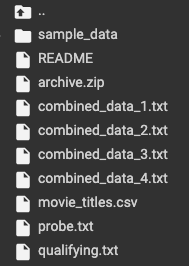
\includegraphics{images/hw1q2.png} \\

Data integrity tends to be a problem in large scale processing, especially if there is little to no support. Therefore, it's important to verify the quality of the file download. 

\noindent
\begin{enumerate}
\item A large part of machine learning and data science is about getting data in the right format. Go ahead and verify the schema and add the screenshots to your assignment.
\end{enumerate}


%%%%%%%%%%%%%%%%%%%%
\subsection{Data Analysis}
\label{sec:data-analysis}
%%%%%%%%%%%%%%%%%%%%

What are some things that we can glean from the data? Let's first try to answer the following questions: 

\begin{enumerate}
    \item Can you plot the distribution of star ratings over users and time?
    \item Are there any trends of star ratings over time?
    \item Are there any films that have gotten more attention over time?
    \item How many films have been re-released? How do you know?
\end{enumerate}

What other information might we try to extract to better understand the data? For the questions that you may come up with (especially any time series data), make sure you back up your assertions with plots. Go ahead and play around with the data, and explore. What are some interesting problems that we may solve? (Without solving it. That's for later in the class!)

\section{Grading Criterion}

A significant portion of the grading rubric is the presentation of your report. We'll review:

\begin{enumerate}
    \item whether or not you've set up your machine in a functional way (15\%).  
    \item the answers to your questions in Sec.~\ref{sec:data-analysis} (35\%).
    \item the clarity of your write-up, including creative solutions (40\%)
\end{enumerate}

Note that there isn't necessarily an absolute \emph{correct} answer to the questions in Sec.~\ref{sec:data-analysis} (though there are certainly \emph{incorrect} answers).

\end{document}

